\documentclass[11pt, oneside]{article}   	% use "amsart" instead of "article" for AMSLaTeX format
\usepackage{geometry}                		% See geometry.pdf to learn the layout options. There are lots.
\geometry{letterpaper}                   		% ... or a4paper or a5paper or ... 
%\geometry{landscape}                		% Activate for for rotated page geometry
%\usepackage[parfill]{parskip}    		% Activate to begin paragraphs with an empty line rather than an indent
\usepackage{graphicx}				% Use pdf, png, jpg, or eps� with pdflatex; use eps in DVI mode
								% TeX will automatically convert eps --> pdf in pdflatex		
\usepackage{amssymb}
\usepackage{amsmath}
\usepackage{algorithm2e}

\title{Notes on Reconfiguration Among Clutter}
%\date{}							% Activate to display a given date or no date

\begin{document}
\maketitle

\section*{Introduction}
In these notes we examine the problem of grasping an object in a cluttered environment.  We categorize the clutter into two groups: static and movable objects. We allow the robot to push any movable object in order to clear a path for grasping the target object.  The robot must avoid contact with static obstacles.  

\section*{Related Work}


\section*{Problem Formulation}
We now provide a more formal description of the problem and introduce notation used throughout the remainder of these notes. As stated previously, we wish to solve the problem of grasping an object, $G$, in a cluttered environment.  Specifically, we say that we have a robot operating in an environment with both static and movable objects.  Let $O = \{O_1, ..., O_k\}$ be the set of static objects.  These objects should be treated as obstacles. Contact between the robot and these objects is forbidden.  Let $M = \{M_1,...,M_n\}$ be a set of movable objects.  These objects can be displaced via contact with the robot. We require that this displacement does not introduce contact between any two objects in $M$ nor does it introduce contact between an object in $M$ and an object in $O$.  Finally, we cannot introduce contact between any object in $M$ and our goal object $G$.  We treat our goal object as a movable object and identify the same contact constraints as any object in $M$, but identify it separately.  We say that a movable object can be displaced when the robot is touching the object.

Let $C_R$ identify the configuration space of the robot.  Let $G_R$ identify the configuration space of the target object, $G$. We can define our goal as a set of configurations, $Q_G = \{q_t \in C_R | f(q_t, g_t) = 0 \}$, where $f(q_t, g_t) = 0$ when our goal object in pose $g_t$ can be stably grasped by the robot in configuration $q_t$.  Let $C_{M_i}$ represent the configuration space of $M_i$.  We can then formalize our problem as follows: given an initial configuration of the robot, $q_0 \in C_R$, an initial configuration of the target object, $g_0 \in G_R$ and an initial configuration for each movable objects, $(c^{M_1}_0,...,c^{M_n}_0) \in (C_{M_1},...,C_{M_n})$, we want to find a path from $q_0$ to any configuration $q_t \in Q_G$ that is collision-free.  

\subsection*{Events}
Here we define the concept of a "contact event."  We define a set of contact indicators, $(I^{M_1},...,I^{M_n}) \in \{0,1\}$ where $I^{M_i} = 1$ if the robot is in contact with movable object $M_i$ and $0$ otherwise.  We can then say a contact event is one where $I^{M_i}_{t-1} \neq I^{M_i}_{t}$ for any $i$.  Informally, we define such an event as any moment in which the contact state between the robot and a movable object changes.  

\subsection*{Actions}
Ultimately we wish to produce a path defined by a sequence of actions, $a_0,...,a_m$ such that when applied to the state $q_0$ the resulting state is a state $q_m \in Q_G$.  We can parameterize these actions as follows:
\[a_t = \left[ \dot{v}, \dot{\theta}, \dot{a}, \Delta t \right] \]
where $\dot{v}$ is the forward velocity of the manipulator, $\dot{\theta}$ is the rotational velocity of the manipulator, $\dot{a}$ is the aperture of the end-effector and $\Delta t$ is the maximum duration of the action.

\begin{figure}[h]
\centering
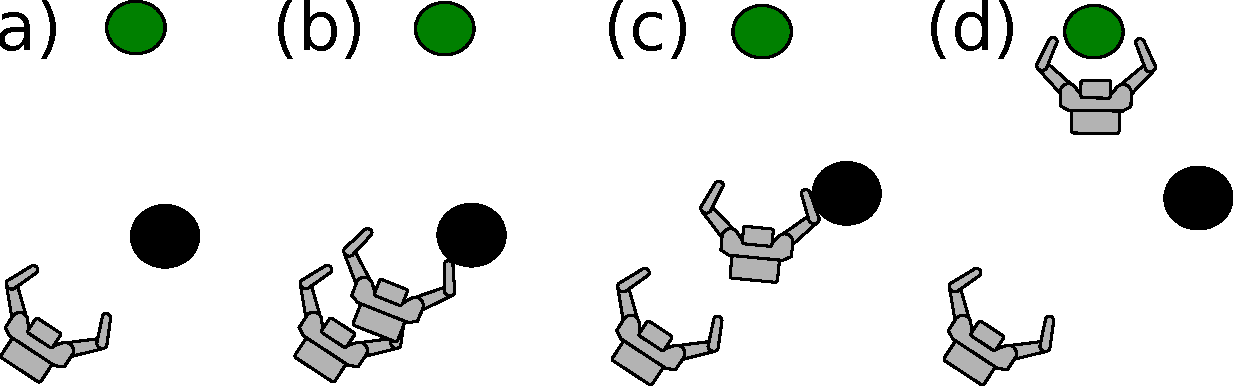
\includegraphics[width=0.8\textwidth]{action_events}
\label{fig:action_events}
\end{figure}
We note that an action can encompass multiple events.  Consider the action depicted in Figure ~\ref{fig:action_events}.  During execution of this action, the robot starts out of contact with any movable obstacle.  The robot then makes contact with obstacle $M_2$, triggering a contact event (Figure ~\ref{fig:action_events}).  After pushing the obstacle out of the way the robot loses contact with the obstacle, triggering a second contact event (~\ref{fig:action_events}).  Thus we can say we have a one-to-many relationship between actions and events.  This will be important during formulation of our algorithm.

\section*{Forward Search}
\begin{algorithm}
\SetKwFunction{ContainsGoal}{ContainsGoal}
\SetKwFunction{Different}{Different}
\SetKwFunction{InitTree}{InitTree}
\SetKwFunction{Sample}{SampleConfiguration}
\SetKwFunction{Nearest}{NearestNeighbor}
\SetKwFunction{Extend}{Extend}
\KwIn{ the start node $q_{init}$ }
\KwOut{ the tree $T$ }
\BlankLine
\SetLine
$T \leftarrow$ \InitTree($q_{init}$) \;
\While{not \ContainsGoal{$T$}} {
$q_{rand} \gets$ \Sample{} \;
$q_{near} \gets$ \Nearest{$T$, $q_{rand}$} \;
$q_{new} \gets$ \Extend{$T$, $q_{near}$, $q_{rand}$} \;
\If{\Different{$q_{new}$, $q_{near}$}} {
$T$.add\_vertex($q_{new}$) \;
$T$.add\_edge($q_{near}$, $q_{new}$) \;
}
}
\label{alg:rrt}
\caption{The basic RRT algorithm}
\end{algorithm}
We can utilize an RRT to perform a forward search through our space starting from the initial state of the environment $q_0$.  The RRT algorithm can be seen in Algorithm ~\ref{alg:rrt}.  During execution of the Extend function, we forward simulate each action starting with the environment in state $q_{near}$ until one of the following stop criteria is encountered:
\begin{enumerate}
\item The simulation time has exceeded the maximum duration, $\Delta t$, defined for the action.
\item The simulation has produced a collision with an obstacle in the environment.
\item The simulation has produced a collision between a movable object and an obstacle.
\item The simulation has produced a collision between two movable objects.
\end{enumerate}
Once the action is stopped, $q_{new}$ will be generated based on the state at that instance in the simulation.
During forward simulation, any contact between the robot and a movable object will trigger the robot to push the object.  We assume quasi-static interactions between the robot and the pushed object.  


The following section provides a brief overview of the physics model that is used.  We note that while this model provides fast forward simulation, it can be replaced by a more detailed physics simulation engine.

\section*{Backward Search}
\begin{figure}[h]
\centering
\label{fig:backwards_search}
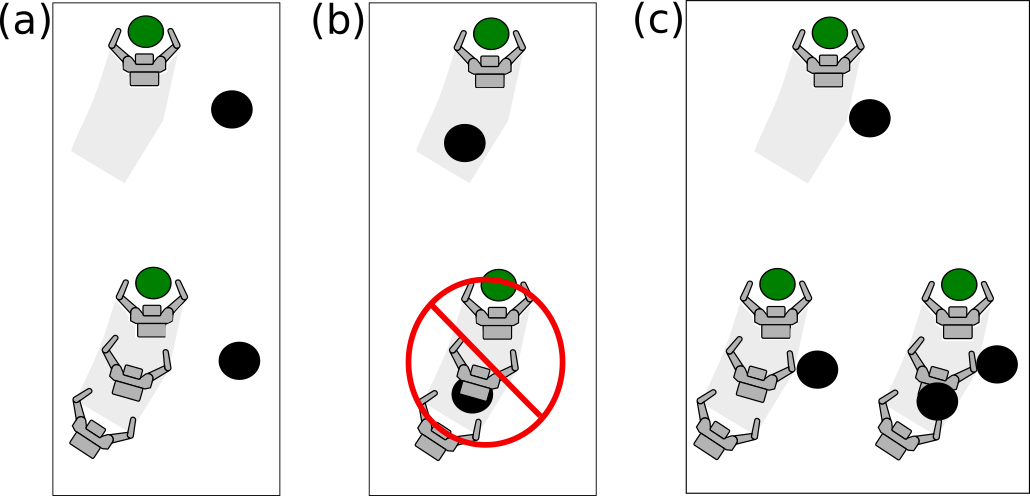
\includegraphics[width=0.8\textwidth]{backwards_search}
\end{figure}
While forward search will allow for generating feasible plans for grasping the object, we wish to speed planning via use of the RRT-Connect planner, which maintains two trees, one grown from the start and one from the goal, and attempts to connect them.  In order to build a tree grown backwards from the goal, we need a method for backwards simulating a pushing action.  Introducing this backwards simulation poses challenges not present in the forward search.  Figure ~\ref{fig:backwards_search} shows the three situations that can be encountered. In the left most figure, backwards simulation of the action shows no intersection between the footprint of the end-effector and the movable object (black circle).  Thus there is a one-to-one mapping between the end-state and the start-state.  In the middle figure, a movable object sits in the footprint of the action.  This renders the action impossible, as there is no way the end-effector could have swept that volume of space without moving the object or having a collision which stopped the action earlier.  The figure on the right shows the most interesting case.  Here there is a movable object that is touching the edge of the swept volume of the end-effector.  This case introduces a one-to-many mapping between the start state and this end state.  Two such mappings are shown in the figure.  The first shows a scene where the object was not pushed during the action, but instead just happened to be sitting on the edge of the action space.  The second shows the object in the swept volume at the start of the action. During execution of the action the object is pushed to the final resting location.  In this case there are an infinite number of possible states that could have started the action.  Each of these states differ only in where the object started, or equivalently where the push would start during action execution.

\begin{figure}[h]
\centering
\label{fig:pre_image}
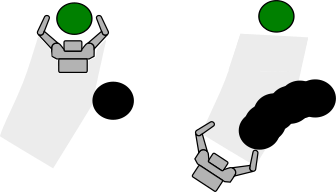
\includegraphics[width=0.8\textwidth]{pre_image}
\end{figure}
In order to enable the use of a bi-directional search strategy, we must decide on a method for handling this ambiguity in the reverse search.  For this we will define the notion of pre-image.  We say the pre-image of an object is the set of all configurations that an object could have started in such that it ended in its final location.  Figure ~\ref{fig:pre_image} shows an example pre-image for an object being pushed.  The pre-image represents every pose for the object from which the push could have started. We then modify our state to represent the pose of a movable object by its pre-image. For the two unambiguous cases in the reverse search (Figure ~\ref{fig:backwards_search}(a)(b)), the pre-image will represent a single pose.  

Using this representation, we can now reduce our infinite number of start locations down to two: the first represents a pure transit by the end-effector, where the object is not pushed.  The second represents the infinite set of transfers. 

\begin{figure}[h]
\centering
\label{fig:example_expansion}
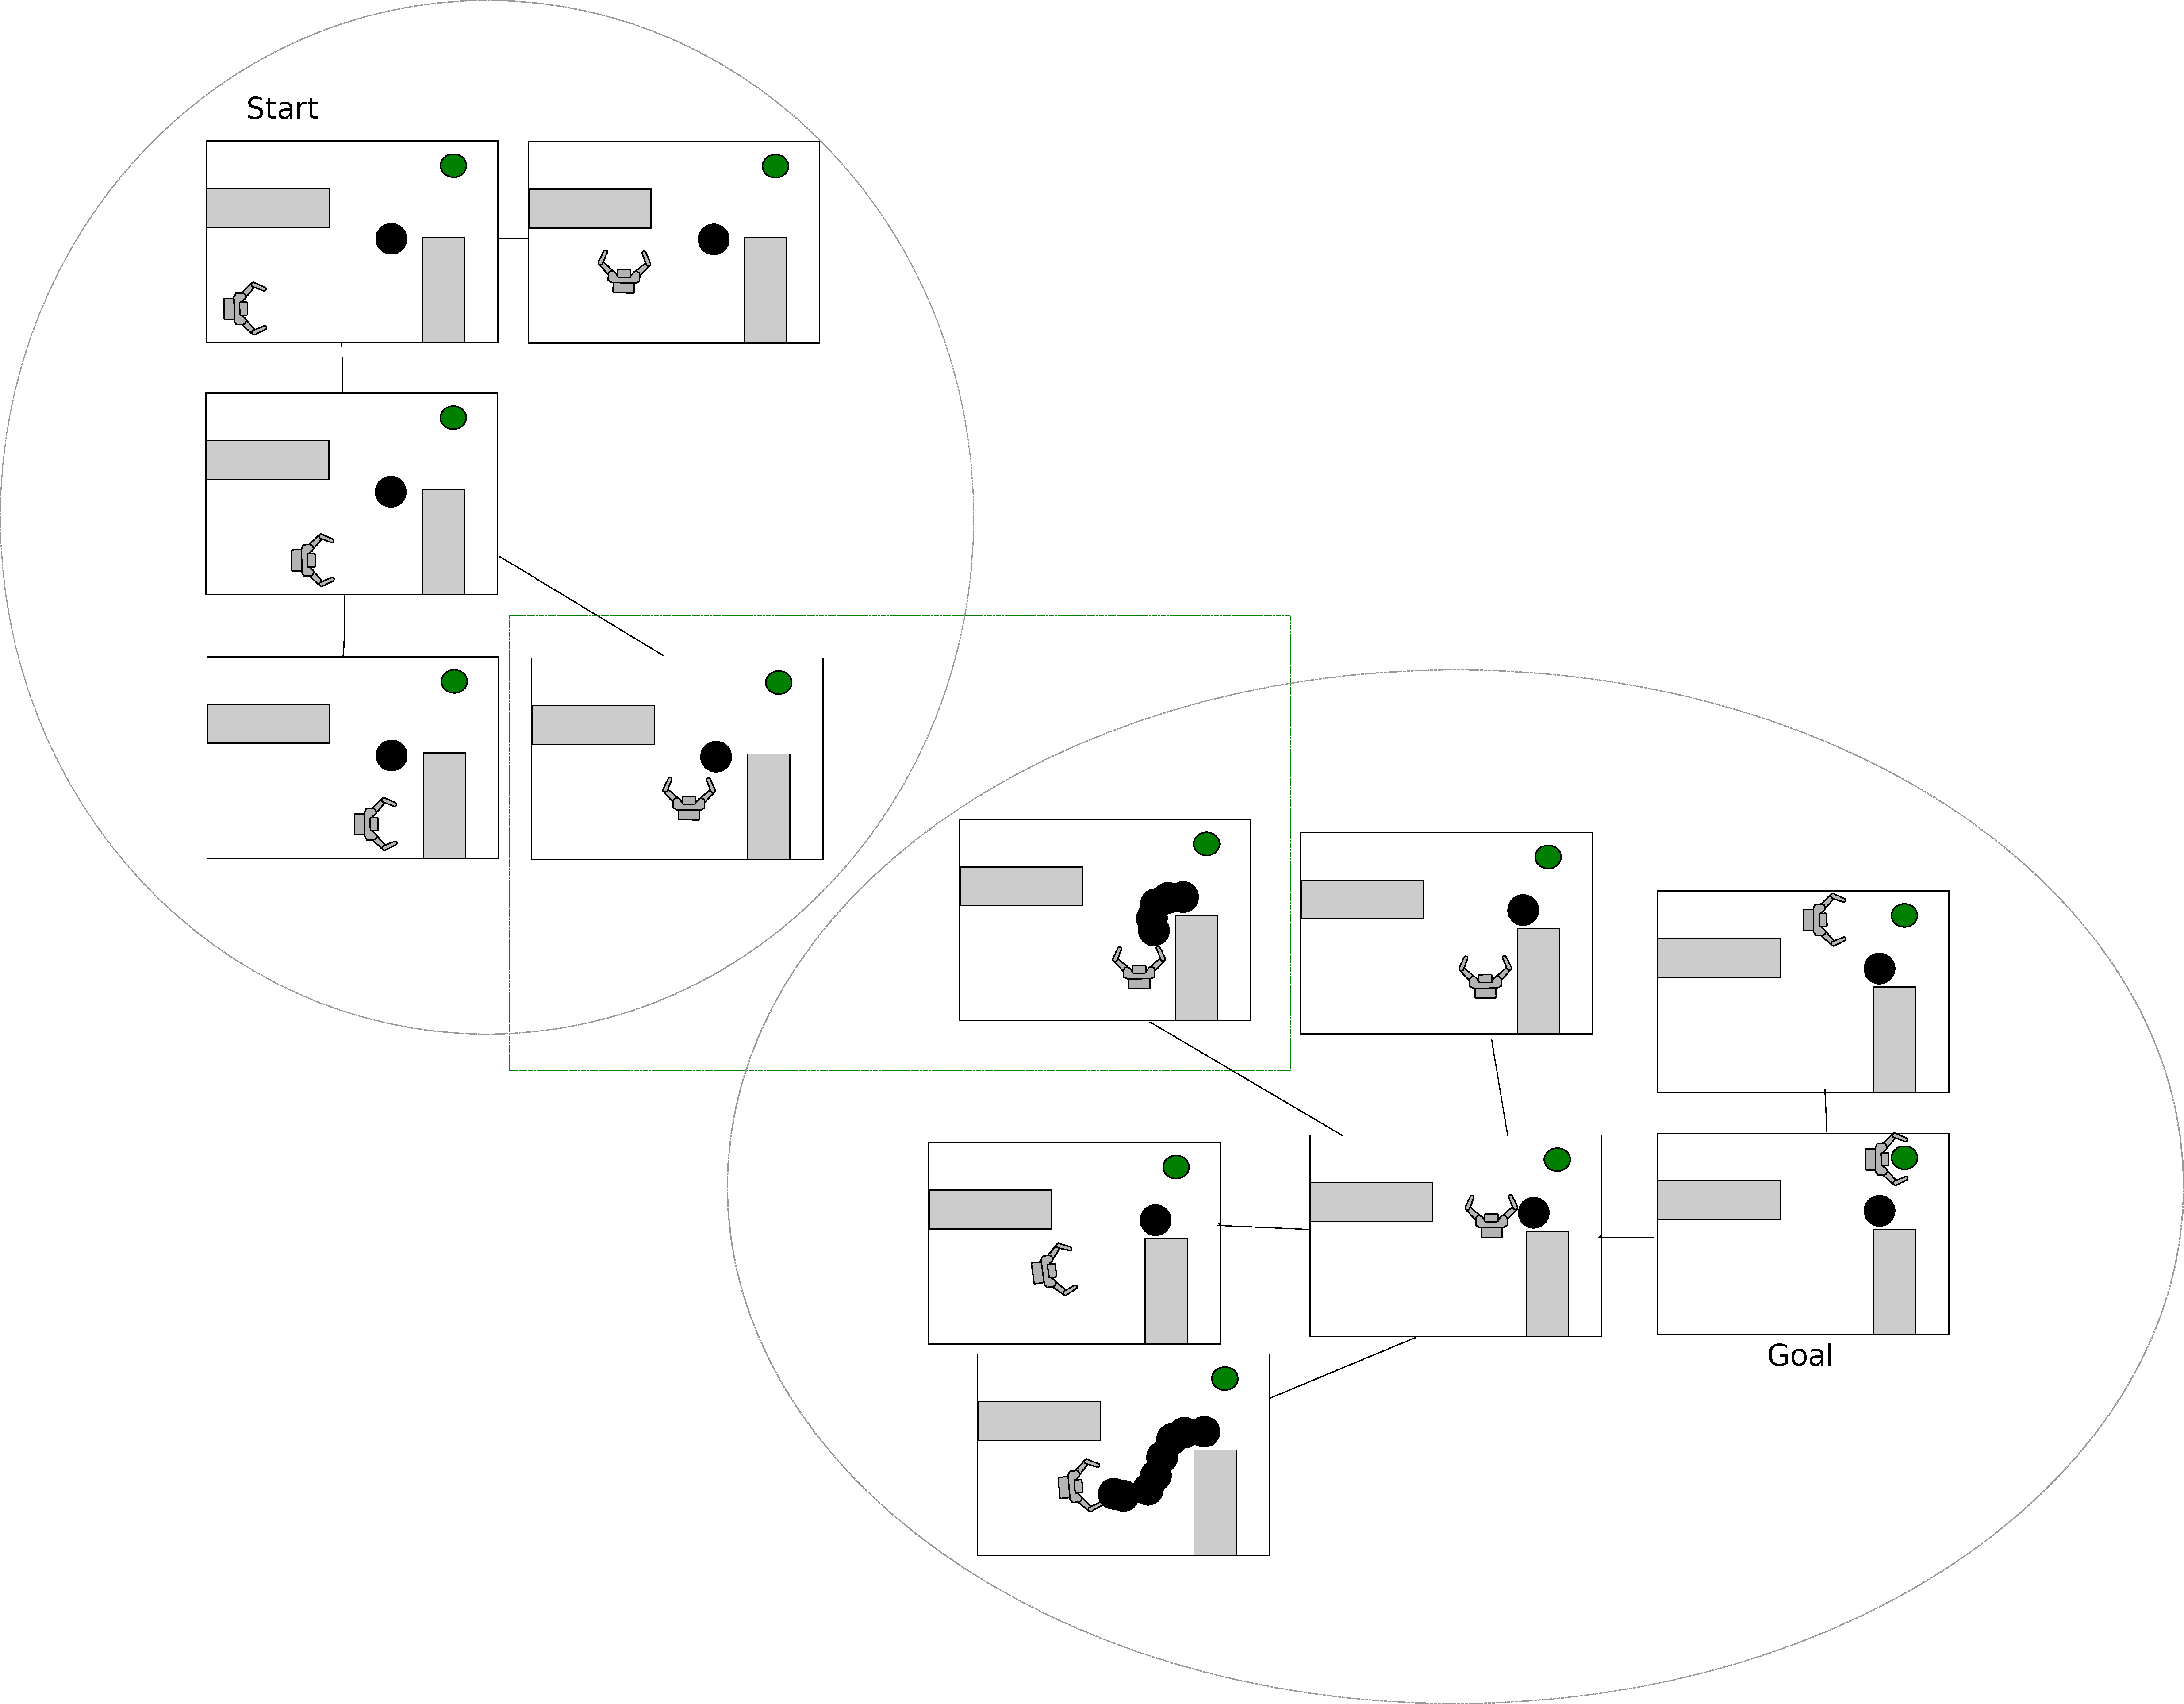
\includegraphics[width=1.0\textwidth]{example_expansion}
\end{figure}
\begin{figure}[h]
\centering
\label{fig:example_solution}
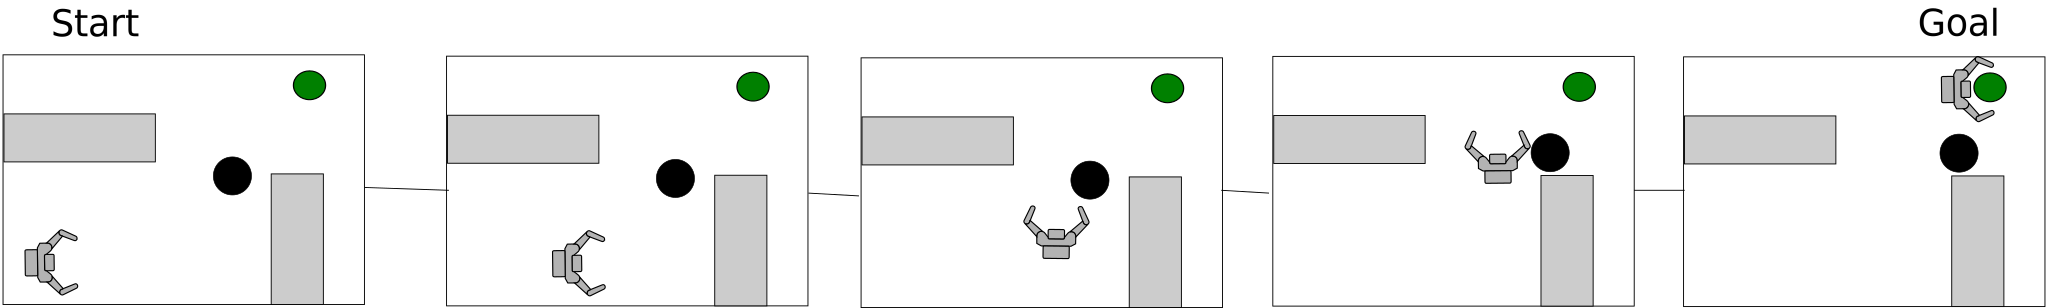
\includegraphics[width=1.0\textwidth]{example_solution}
\end{figure}
Figure~\ref{fig:example_expansion} shows growth of the bi-directional search tree for a simple problem.  The two states in the green box in the center of the figure represent equivalent states.  Thus the trees meet when these two states are added to their appropriate subtrees. Figure~\ref{example_solution} represents the final path generated by the search.

\end{document}
